\section{Methods}

\subsection{Overview}

Our hypothesis is that performing test time adaptation on cell segmentation will improve cell tracking performance since the associations are based on simple metrics such as IoU and Euclidean distance of the centroids. We propose to pretrain a denoising framework that takes three inputs: The raw image, noisy segmentation from a pretrained segmentation model, and Gaussian splats retrieved from the raw image, and produce a clean segmentation mask as pseudo labels.
Once the pseudo labels are retrieved, we perform knowledge distillation with stochastic restoration of parameters to perform the test-time adaptation. Please refer to \Cref{fig:overall_framework}.


\begin{figure}[t]
    \centering
    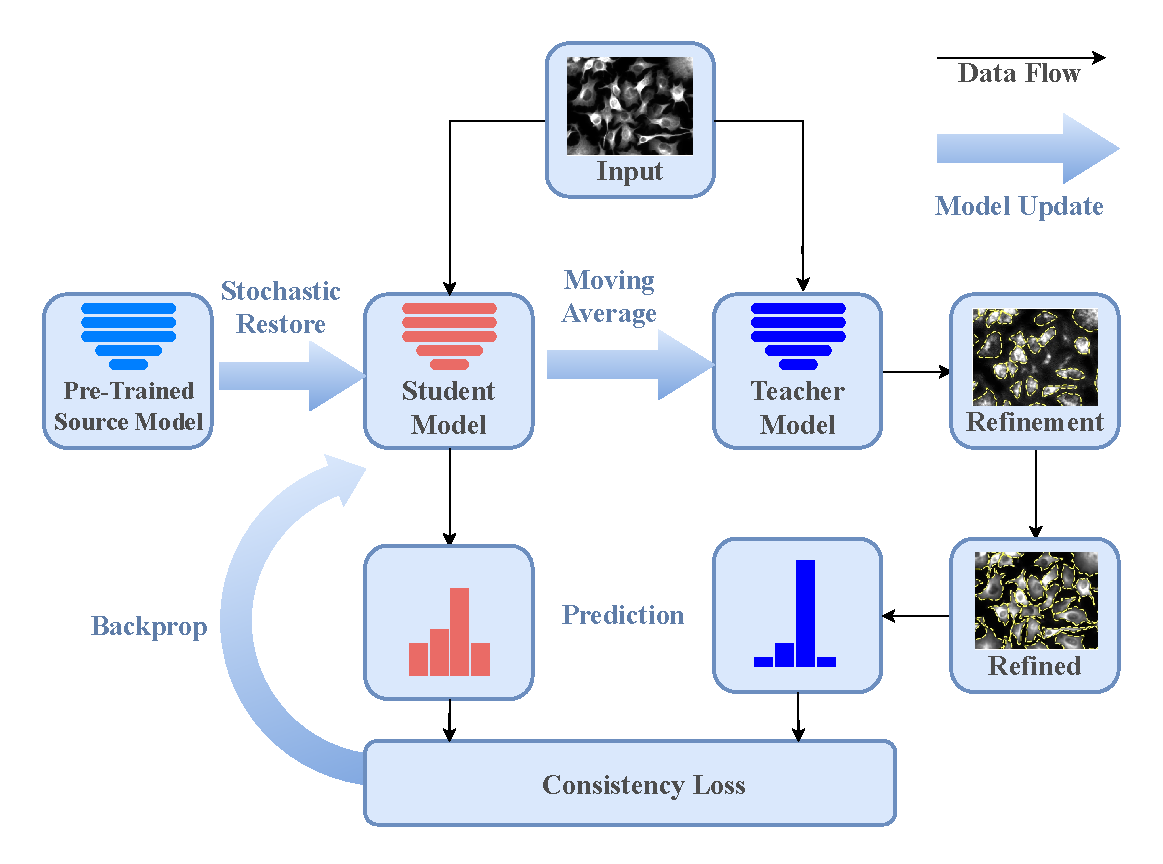
\includegraphics[width=9cm]{figs/project_proposal.pdf}
    \caption{Overall Framework.}
    \label{fig:overall_framework}
\end{figure}

\subsection{Cell Segmentation}

To test our hypothesis, we use one of the state-of-the-art cell instance segmentation algorithms as our segmentation framework Cellpose~\cite{stringer2021cellpose}. It is pretrained on diverse datasets and has good generalization capability. However, it is not pretrained on all imaging modalities or cell types, rendering it less useful in out-of-distribution datasets. We propose to utilize their pretrained model and perform test-time adaptation. 

Here, we describe the inner workings of Cellpose~\cite{stringer2021cellpose}: given an image $I$, the model uses a network $f$ to produce a dense, pixel-wise feature $\bm{Z} = f(I)$, where $ \bm{Z} = [Z_1, Z_2, Z_3] \in \mathbb{R}^{h \times w \times 3}$. Given the feature $\mathbf{z} = [z_1, z_2, z_3] \in \bm{Z}$ for some pixel $i$, then $\bm{z} \doteq (z_1, z_2)$ has the meaning of gradient pointing towards the center of the cell structure to which pixel $i$ belongs. Collectively, $(Z_1,Z_2)$ form a \emph{gradient flow}. Instead, $z \doteq z_3$ represents the unnormalized score indicating the probability of pixel $i$ to belong to a cell structure. Note that with this notation, the feature $\mathbf{z}$ can be written as $\mathbf{z} = [\bm{z}, z]$. The network $f$ is trained in a supervised manner with pixel-wise instance segmentation loss
\begin{equation}
  \mathcal{L}_i^{IS} = (z_1 - \mathtt{g_x})^2 + (z_2 - \mathtt{g_y})^2 + \nu H(\mathtt{m},\sigma(z))  \; ,
\end{equation}
where, for pixel $i$,  $(\mathtt{g_x}, \mathtt{g_y})$ represents the ground-truth gradient label with unit $\ell_2$-norm, $\mathtt{m} \in \{0, 1\}$ is the binary mask label indicating absence/presence of a cell structure, $\sigma(z) \doteq 1/(1+\exp(-z))$, $H$ represents the binary cross-entropy, and $\nu$ is a hyperparameter set to $0.04$. The pixel-wise loss contributions are then aggregated into a final loss $\mathcal{L}^{IS} = \sum \mathcal{L}_i^{IS}$ for the image $I$.


Given the feature $\bm{Z}$, the cell instance segmentation head $g$ produces the mask $Y = g(\bm{Z})$, where for pixel $i$, the predicted label $y$ is a number in the set $\{0, 1, \cdots, N \}$, with $N$ being the total number of cell instances segmented. Pixels belonging to the same cell instance have same label, and $y=0$ indicates absence of a cell instance.


\subsection{Training Gaussian Splats Algorithm}

Radiance fields are a new form of 3d representation which relies on novel differentiable ray-marching, in this talk we will discuss two types Neural Radiance Fields (NeRF) and Gaussian Splatting (GS).   In brief, a radiance field is a learnable representation of a scene, in the case of the NeRFS a large MLP is used as the mechanism and in GS a variable list of ellipsoids.  A raycast is a form of graphics rendering in which the emission of photons onto a pixel is calculated by tracking the reflection of light.  For instance, to find the color of the middle pixel of an image, a ray can be calculated in the opposite direction of how light is received by the camera.  Usually in the case of raycast, for simplicity, once the ray hits an object in the 3d scene it stops and the color of the hit object is blended into that pixel.  \\

Instead of the ray cast ending after an arbitrary number of reflections, the rays’ direction is not affected by reflection.  Each perceptron in NeRF or Ellipsoid in GS is associated with an emission of light which adds its contribution to the ray by integrating the contribution of each perceptron or ellipsoid to the ray small changes to the light emitted are captured by the alpha-blending equation. Each of these are trained by taking training samples and finding the divergence between the rendering at the current training step compared to the known ground truth image.  In order, to have this information though you need to also know the pose of the camera relative to the scene during training which can be a major impediment to applying a radiance field method. In this case we have the benefit of a closed system where we can define the position of the viewer based on the geometry of the original imaging system which is published information.  \\

\subsection{Refinement}
The refinement module processes three inputs to construct a more refined mask. These three inputs are: the raw image volume, initial segmentation produced by the Cellpose~\cite{stringer2021cellpose} base model, and Gaussian splats constructed from the raw image volume. On the architecture side, this module shares the exact same architecture as CellpoSe~\cite{stringer2021cellpose}, except the number of input channels. Please refer to ~\Cref{fig:refinement}.

\begin{figure}[t]
    \centering
    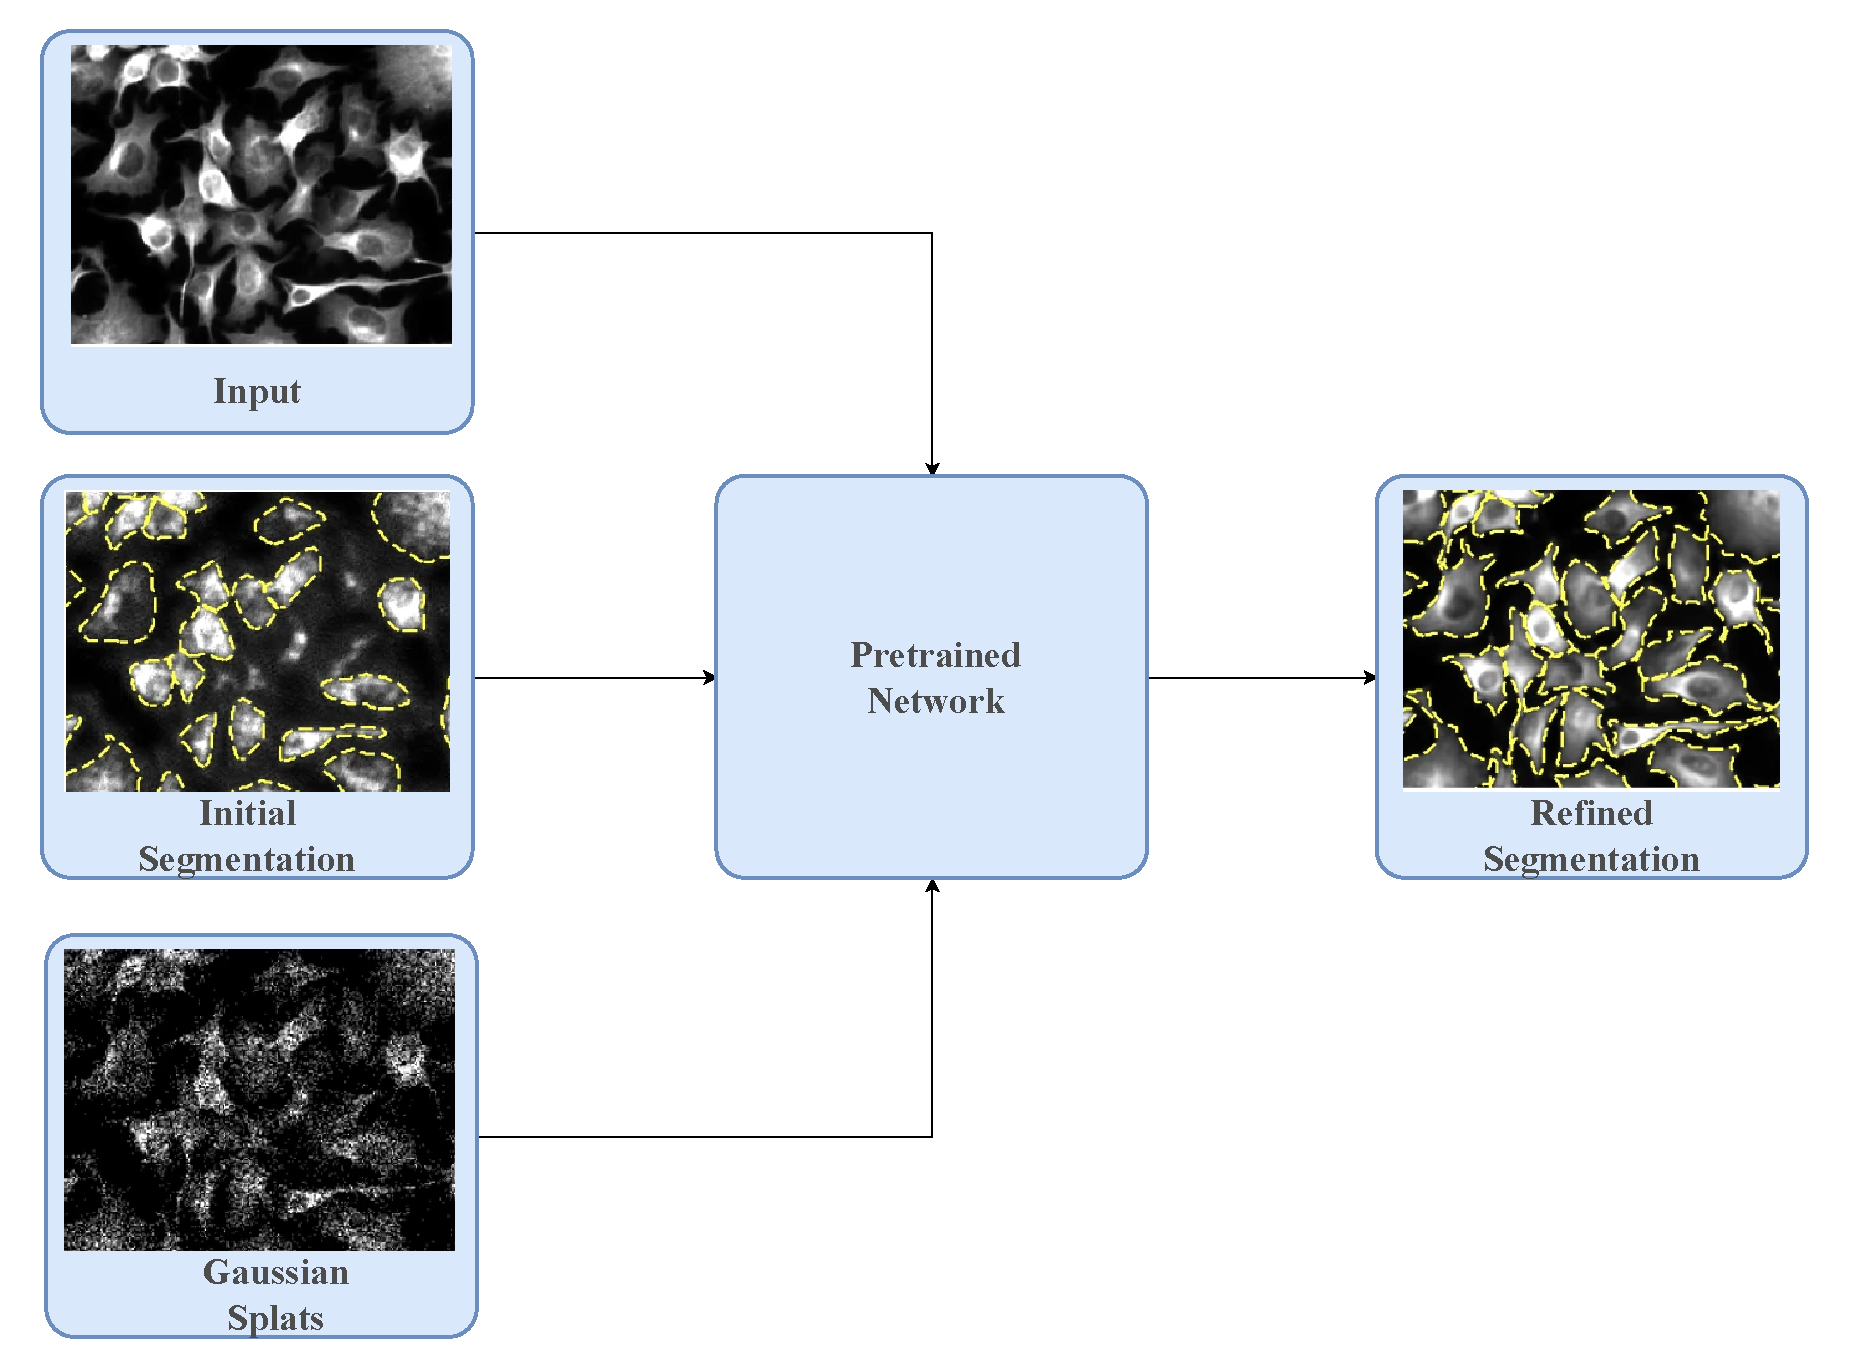
\includegraphics[width=9cm]{figs/refinement.pdf}
    \caption{Refinement Strategy.}
    \label{fig:refinement}
\end{figure}

\subsection{Test-Time Adaptation}
Please refer to the schematic in \Cref{fig:overall_framework} for a general overview of our approach. The pretrained cell segmentation model by Cellpose~\cite{stringer2021cellpose} will be the source model. We will make two copies of the source model: the student and the teacher model. A raw input, i.e., microscopy image volume, will be fed to the student as well as the teacher model. The output from the teacher model will be combined with the raw image volume and the Gaussian splats and will be fed to the pretrained refinement module. The prediction from the refinement module will be used as the pseudo labels and a consistency loss will be employed to perform the back propagation on the student model. A stochastic restoration procedure proposed in \cite{wang2022continual} will be used to restore parameters from the original source model. We will then update the teacher model with a moving average of the parameters.    \\


Update on the teacher model is given by
\begin{align}
    \theta'_{t+1} = \alpha \theta'_{t} + (1-\alpha)\theta'_{t+1},
\end{align}


The stochastic restoration of the parameters is given by
\begin{align}
    M &\sim \text{Bernoulli}(p), \\
    W_{t+1} &= M \odot W_0 + (1-M) \odot W_{t+1}, 
\end{align}
where $W$ are the parameters. \\



\subsection{Cell Tracking}
\dots